\section{Entwicklung des Gesamtkonzepts} \label{sec:Meth gesamtkonzept}
Um ein Gesamtkonzept für das \gls{Modul} zur automatischen Verhaltensklassifikation zu entwerfen, sind einige grundlegende Aspekte zu betrachten. Zentral ist die Definition der Aufgabe, die mittels maschinellem Lernen gelöst werden soll. Diese ist aus den Anforderungen an das \gls{Modul} abzuleiten. Ebenfalls ist die Rohdatengrundlage zu betrachten, aus welcher sich die Erfahrung, in Form von Features extrahieren lässt. Über die Rohdatengrundlage ist der Moduleingang bestimmbar. In diesem Kapitel werden deshalb die Modulanforderungen betrachtet und die Rohdatengrundlage und Voraussetzungen. Anschließend wird die maschinelle Lernaufgabe definiert. Die Erkenntnisse fließen in einem Gesamtkonzept für das Modul zusammen. Bezogen auf den \gls{Machine Learning Workflow} (\autoref{sec:MLWF}), wird hier auf  die \textit{Problemdefinition} und die Vorbereitung für das \textit{Sammeln von Daten} beschrieben. \par


\subsection{Anforderungen an das Modul} \label{sec:Meth Anforderungen}

Aus den Zielsetzungen für die Modul-Entwicklung (\autoref{sec:Zielsetzung}) lassen sich Anforderungen ableiten. Da explizit maschinelles Lernen verwendet werden soll, grenzt dieses Ziel die Methodenauswahl ein. Durch diese Eingrenzung, ist abzuleiten, dass Features zu extrahieren sind und ein maschinelles Lernmodell benötigt wird. Da Verhalten erkannt werden soll, steht fest, dass das Modell ein \gls{Klassifikation}[sproblem] lösen muss. Das grenzt die Methodenauswahl weiter ein. \par

 Das Konzept soll modular sein. Es muss sich einfach in eine Datenverarbeitungskette integrieren lassen, um für übergeordnete Systeme nutzbar zu sein. Dafür muss es ebenfalls Verhalten automatisiert auswerten. Eine manuelle Steuerung ist nicht erwünscht. Die Verarbeitung soll nur einen Datenstrom als Eingang erhalten, aus vorausgegangenen Modulen in der Verarbeitungskette. Aus dem Ziel der Echtzeitfähigkeit ergeben sich Anforderungen an die Laufzeit. Diese muss so kurz sein, dass sich nach Eintreffen des Ergebnisses noch Einfluss auf das Verhalten nehmen lässt. Die Verarbeitungsdauer des Moduls muss somit möglichst kurz sein. \par

 Neben der Zielsetzung ist der Zeitrahmen ein einschränkender Faktor. Um eine erfolgreiche Entwicklung in der vorgegebenen Zeit zu gewährleisten, muss der Implementierungsaufwand von Modul und maschinellem Lernmodell realisierbar sein. In Bezug auf das Gesamtkonzept wirkt sich dieser Fakt primär auf die Feature-Extraktion, Konstruktion und die Modellauswahl aus. Modelle, die komplex zu implementieren sind, können dadurch ungeeignet sein. Das Gleiche gilt für besonders komplexe Features.



\subsection{Rohdatengrundlage und Voraussetzungen} \label{sec:Meth RohDat}
Die Rohdaten sind fundamental für den Aufbau von Anwendungen des \glsdisp{ML}{maschinellen} Lernens. Im \gls{Machine Learning Workflow} wird sich ab dem zweiten Prozessschritt mit ihnen auseinandergesetzt (\autoref{sec:Worflow DatSam}). Die frühe Position im Ablauf zeigt, dass sämtliche folgenden Prozesse auf den Rohdaten fußen. Eine frühzeitige Bestandsaufnahme der zur Verfügung stehenden Rohdaten kann einen erfolgreichen Verlauf des Workflows gewährleisten. \par

Im \acrshort{OptiLiMa} Projekt wurden Rohdaten aus einem Mastputenstall gesammelt. Dieser wurde mit zwölf Kameras ausgestattet, die jeweils einen anderen Stallbereich abdeckten. Positioniert wurden die Kameras so, dass sie das Stallgeschehen aus der Vogelperspektive aufzeichneten. Die Abbildung \ref{fig:KamerasImStall} stellt die Einteilung des Mastputenstalls in die mit Kameras abgedeckten Bereiche dar. Eingezeichnet ist der ungefähre Verlauf der Futterbahnen.

\begin{figure}[htb]
    \centering
    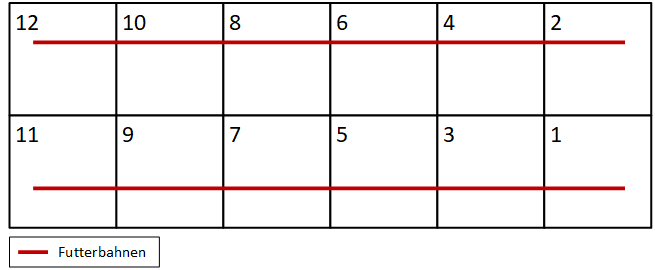
\includegraphics[width=0.9\textwidth]{img/Grafiken/Stallbereiche mit Futterbahn.png}
    \caption[Abteile des Mastputenstalls mit Verlauf der Futterbahnen.]{Abteile des Mastputenstalls mit Verlauf der Futterbahnen. Die Nummer in den oberen linken Ecken stehen für die IDs der Kameras.}
    \label{fig:KamerasImStall}
\end{figure}

Die Kameras nahmen einen Videostream auf. Die Bildinformationen wurden verwendet, um ein \gls{Detektion}[s]\glsdisp{Modul}{modul} anzuwenden. Dieses \glsdisp{Detektion}{detektierte} und \glsdisp{Lokalisation}{lokalisierte} die Puten im \gls{Frame}. Die \gls{Detektion} verlief in Echtzeit. Die \gls{Detektion}[en] wurde in einer Datenbank gespeichert, die sich auf einem Server befindet. Jeder Eintrag beinhaltet einen eindeutigen Zeitstempel und ein dazugehöriges \gls{Frame} in einem Videostream. Die Videostreams wurden auf Festplatten gespeichert. Insgesamt wurden  drei Mastdurchläufe aufgezeichnet. Ein Lebenszyklus der Puten umfasst ca. 4 Monate. Nach einer Aufzuchtphase von einem Monat kommen die Tiere in den Mastputenstall. Ab diesem Punkt begann die Datenerfassung. \par

Die Datensammlung im Mastputenstall war bereits vor Beginn dieser Arbeit abgeschlossen. Somit ließ sich kein Einfluss auf die Art und die Menge der zur Verfügung stehende Rohdaten nehmen. Die Videostreams liegen im mp4-Dateiformat vor. Das direkte Arbeiten auf der Datenbank mit den \gls{Detektion}[en] ist wegen des Datenvolumens und der Rechenleistung der Server nicht praktikabel. Aus diesem Grund wurde ein Tool entwickelt, das auf die Datenbank zugreift und Daten eines angegebenen Zeitintervalls herunterlädt. Die heruntergeladenen \gls{Detektion}[en] speichert das Tool in einer csv-Datei. In einer vorausgegangenen Arbeit im Rahmen des \acrshort{OptiLiMa} Projekts wurde ein \gls{Assoziation}[s]\glsdisp{Modul}{modul} entwickelt, das die \gls{Detektion}[en] nutzt. Somit steht ein \gls{MOT} System zur Verfügung. \par

Die \gls{Detektion} und die \gls{Assoziation} bauen auf dem Videostream auf. Jedes \gls{Frame} im Videostream hat einen eindeutigen Zeitstempel zugeordnet. Dadurch wird ersichtlich, dass die vorhandenen Rohdaten in Form von Zeitreihen vorliegen.

\subsection{Definition der Aufgabe} \label{sec:Meth DefAufgabe}
Ziel ist es, Verhaltensweisen der Mastputen zu klassifizieren (\autoref{sec:Zielsetzung}). Um eine Aufgabe zu formulieren, muss zunächst geklärt werden, was eine Verhaltensweise ist und wie sie sich erkennen lässt. In \cite{Levitis.2009} wird Tierverhalten definiert als Reaktionen von Individuen oder Gruppen auf Reize aus ihrer Umgebung. Das Suffix \textit{-weise} oder \textit{-art} bezeichnet eine Gewohnheit \cite{duden.art}. Eine Verhaltensweise ist somit ein Muster im Verhalten. Im Vorfeld dieser Arbeit wurden zwei Verhaltensweisen identifiziert, die besonders herausstechen. Diese werden hier als Kontrollgänge und Kämpfe bezeichnet. Im Folgenden werden diese beiden Verhaltensweisen erläutert. \dubpar

\begin{quote}

\textbf{Kontrollgänge}\par
Der Tierhalter unternimmt täglich Kontrollgänge im Maststall. Die Tiere reagieren auf den Tierhalter, wenn dieser den Stall betritt und umhergeht. Dabei finden Massenbewegungen statt. Die Tiere werden aufgeschreckt und fangen an, sich in Richtung des Tierhalters zu drängen. Oftmals beruhigen sich die Tiere noch während des Kontrollgangs. Nähert sich der Tierhalter ihrem Stallbereich, werden sie jedoch oftmals wieder aufgeschreckt und drängen sich erneut in seine Richtung. In seiner unmittelbaren Nähe weichen ihm die Tiere aus. Dadurch entsteht eine \gfuss{Traube} um den Tierhalter. Regelmäßig muss im Stall neues Stroh gestreut werden. Dafür fährt ein Traktor durch den Stall. Das Verhalten der Tiere ist in diesem Fall jedoch sehr ähnlich zum täglichen Kontrollgang. Die Tiere drängen zum Traktor. Um den Traktor bildet sich ein \gfuss{Traube}. Die \gfuss{Traube} ist dabei deutlich größer, aufgrund der Größe des Traktors. Fährt der Traktor durch den Stall, bleibt hinter ihm eine große freie Fläche zurück. Einige Puten nutzen diese Fläche, um dem Traktor nachzujagen. Teileweise füllt sich die Fläche jedoch nur gemächlich. Die Abbildung \ref{fig:bspKontrollg} zeigt einige Ausschnitte aus Kontrollgängen. 
\end{quote}


\begin{figure}[htb]
     \centering
     \begin{subfigure}[b]{0.4\textwidth}
         \centering
         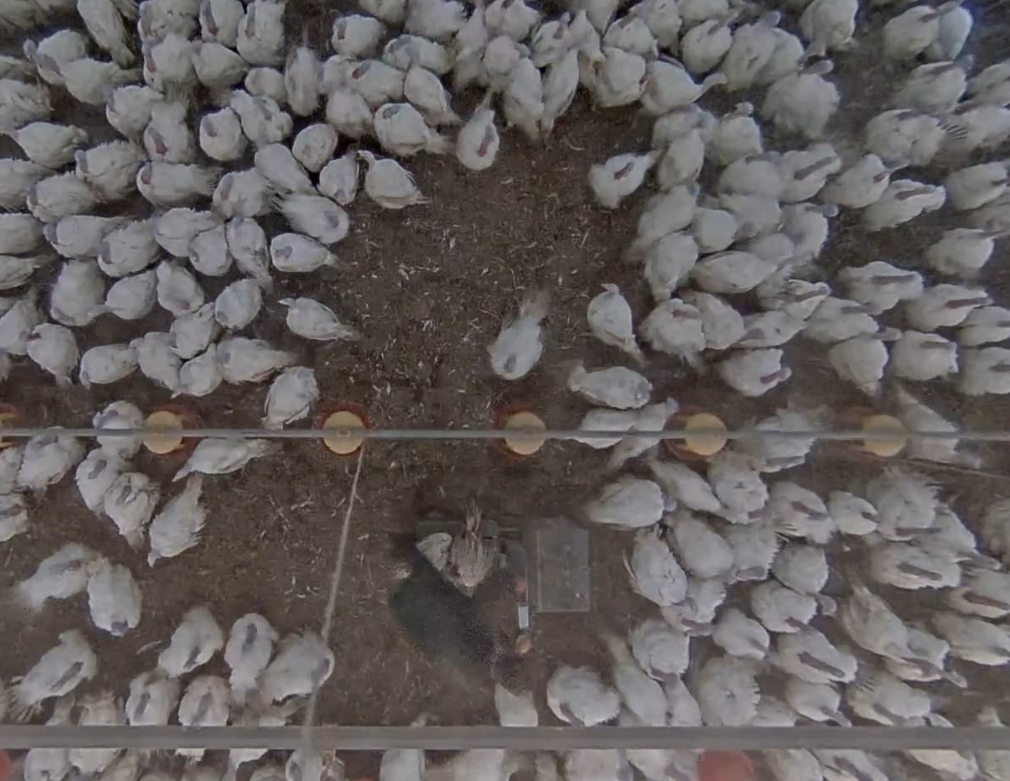
\includegraphics[width=\textwidth, height=5cm]{img/Verhaltensweisen/Kontrollgang Tierhalter Traube 2.png}
         \caption{Kontrollgang des Tierhalters.}
     \end{subfigure}
     \hfill
     \begin{subfigure}[b]{0.59\textwidth}
         \centering
         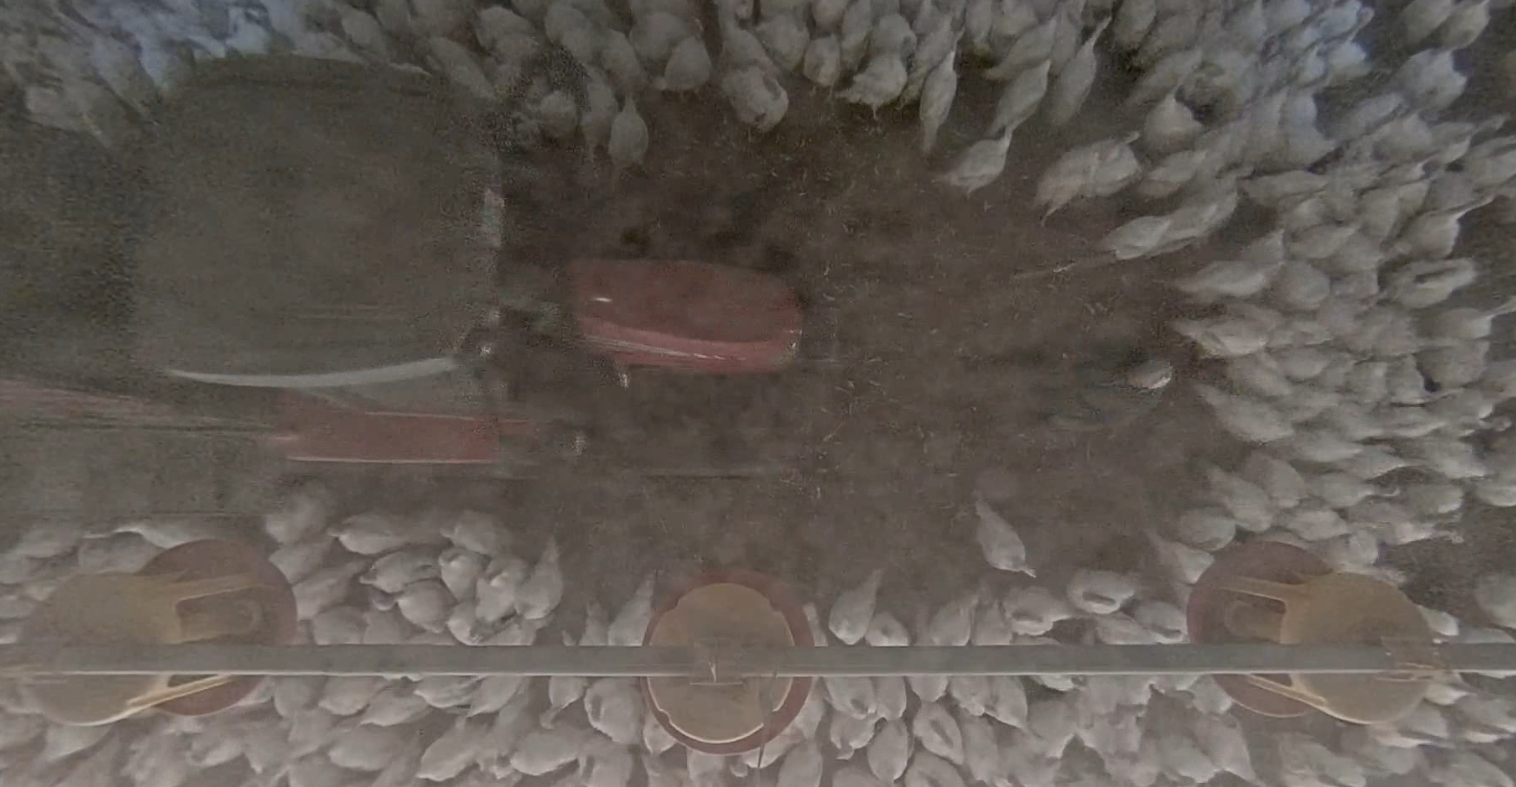
\includegraphics[width=\textwidth, height=5cm]{img/Verhaltensweisen/Kontrollgang Tracktor Traube.png}
         \caption{Einstreuung von Stroh mit Traktor.}
     \end{subfigure}
     \caption[Ausschnitte aus Kontrollgangereignissen.]{Ausschnitte aus Kontrollgangereignissen.}
     \label{fig:bspKontrollg}
\end{figure}


\par

\begin{quote}
\textbf{Kämpfe}\par
Ein Kampf entsteht ohne direkt ersichtlichen Auslöser. Ein Kampf beginnt meistens, indem sich zwei Tiere gegenüberstehen und sich gelegentlich versuchen anzupicken. Dies steigert sich meistens zu stärkeren Pickattacken. Dabei entwickeln die Tiere eine hohe Dynamik und bewegen sich umeinander. Oft passiert es, dass eine Pute die andere packt und um sich schleudert. Dadurch entstehen zirkulierende Bewegungsmuster. Die umliegenden Puten weichen den kämpfenden Tieren aus, wodurch eine \gfuss{Traube} entsteht. Auch Verfolgungen sind zu beobachten. Möchte eins der Tiere entkommen, jagt das andere diesem hinterher. Schafft es der Verfolger, die flüchtende Pute zu packen, wird der Kampf fortgesetzt. Die Verfolgungen finden mit hoher Dynamik statt. Es entstehen freie Flächen im Kanal der Fluchtbewegung. Ein Kampf muss nicht nur zwischen zwei Tieren stattfinden. Auch mehrerer Tiere können an einem Kampf beteiligt sein. Ebenfalls können die kämpfenden Tiere wechseln. Schafft es ein Tier zu flüchten und der Verfolger findet dieses nicht mehr, kann es sein, dass der Verfolger auf das nächstbeste Tier losgeht. Auch kann ein bisher unbeteiligtes Tier sich dazu entscheidet, in den Kampf mit einzusteigen. Der Kampf endet plötzlich und so, wie er begonnen hat, ohne ersichtlichen Auslöser. Die Abbildung \ref{fig:bspKämpf} zeigt einige Ausschnitte aus Kämpfen.
\end{quote}

\begin{figure}[htb]
     \centering
     \begin{subfigure}[b]{0.55\textwidth}
         \centering
         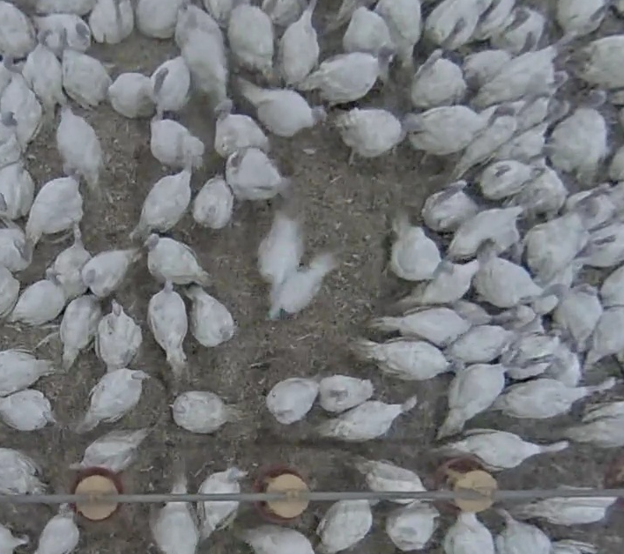
\includegraphics[width=\textwidth, height=6cm]{img/Verhaltensweisen/Kampf Traube.png}
         \caption{Kampf zwischen zwei Puten.}
     \end{subfigure}
     \hfill
     \begin{subfigure}[b]{0.44\textwidth}
         \centering
         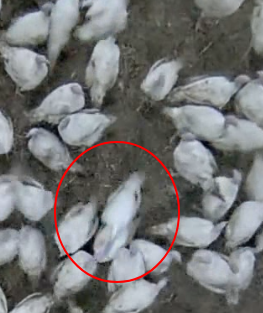
\includegraphics[width=\textwidth, height=6cm]{img/Verhaltensweisen/Kampf Verfolgung.png}
         \caption{Verfolgung eines flüchtenden Tieres.}
     \end{subfigure}
     \caption[Ausschnitte aus Kampfereignissen.]{Ausschnitte aus Kontrollgangereignissen.}
     \label{fig:bspKämpf}
\end{figure}

\par

Bei einem Kontrollgang treten dynamische Gruppenbewegungen auf, während Kämpfe durch dynamische Bewegungen vereinzelter Tiere geprägt sind. Bezogen auf den Kameraausschnitt ist bei einem Kontrollgang Dynamik in den meisten Bildbereichen zu beobachten. Kämpfe fallen durch lokale Dynamik in vereinzelten Bildbereichen auf. \par

Für diese Arbeit wurde jegliches Verhalten, was kein \textit{Kontrollgang} oder \textit{Kampf} ist, als \textit{Normalverhalten} deklariert. Der Begriff ist etwas irreführend gewählt, da \gfuss{Normalität} nicht näher definiert wurde. Jedoch sind Kämpfe und Kontrollgänge die auffälligsten Verhaltensweisen. Ebenfalls sind sie unerwünscht (\autoref{sec:Hintergrund}), weshalb der Fokus darauf gelegt wird, diese Verhaltensweisen vom restlichen Verhalten abzugrenzen. Das restliche Verhalten wird als \gfuss{Normal} bezeichnet. Die Definition der Merkmale von \textit{Normalverhalten} lässt sich aus diesem Grund als Abgrenzung von den anderen beiden Verhaltensweisen Formulieren.\dubpar

\begin{quote}
\textbf{Normalverhalten}\par
Während sich ein Kontrollgang durch eine globale hohe Dynamik auszeichnet und ein Kampf durch lokale hohe Dynamiken, so sind die Puten die meiste Zeit deutlich weniger aktiv. Bezogen auf die Bildbereiche der Kameras ruht sich ein Großteil der Tiere aus. Die Tiere sitzen stationär auf einer Position. Vermehrt tritt Aktivität rund um die Futterbahnen auf. Diese ist jedoch meistens nicht so dynamisch, wie in den anderen Verhaltensweisen.
\end{quote}
\par

Das Auftreten einer Verhaltensweise stellt für das geplante \gls{Modul} ein \gls{Ereignis} dar. Wie die Beschreibungen der Verhaltensweisen zeigen, basieren die charakterisierenden Merkmale vor allem auf der Bewegung der Tiere. Bewegung ist zeitabhängig. Die Merkmale der Verhaltensweise sind somit in einem Zeitraum zu beobachten. Ein \gls{Ereignis} wird also definiert durch einen Startzeitpunkt und einen Endzeitpunkt. Innerhalb dieser zeitlichen Grenzen sind die Merkmale der jeweiligen Verhaltensweise zu beobachten. \par

Aus den Anforderungen (\autoref{sec:Meth Anforderungen}) ist bekannt, dass ein \gls{Klassifikation}[sproblem] zu lösen ist. Durch die Erkenntnis, dass sich die \gls{Ereignis}[se] innerhalb eines Zeitraums abspielen und dem Fakt, dass auch die Rohdaten in Zeitreihen strukturiert sind (\autoref{sec:Meth RohDat}) wird deutlich, dass es sich bei der Aufgabe um eine \gls{Klassifikation} von Zeitreihen handelt.\par

\subsection{Aufbau des Gesamtkonzepts}
Die Aufgabe wurde definiert, die Rohdaten sind bekannt, das Format und die Merkmale der Verhaltensweisen wurden untersucht und die Modulanforderungen wurden formuliert. Mit diesem Wissen ist ein Gesamtkonzept für das \gls{Modul} zu entwicklen. Die Abbildung \ref{fig:GesKonzpt} zeigt dieses Konzept.

\begin{figure}[htb]
    \centering
    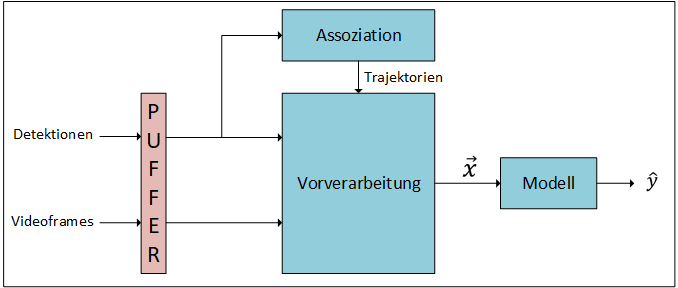
\includegraphics[width=0.9\textwidth]{img/Grafiken/Gesamtkonzept start.png}
    \caption{Gesamtkonzept des \gls{Modul}[s].}
    \label{fig:GesKonzpt}
\end{figure}


Ein Strom von Rohdaten fließt in das \gls{Modul}. Die \gls{Detektion}[sdaten] werden dem \gls{Assoziation}\glsdisp{Modul}{smodul} übergeben. Dieses generiert Trajektorien. Die Rohdaten und die Trajektorien fließen in einer Vorverarbeitung zusammen. Hier werden die \gls{Feature}[s] aus den Rohdaten extrahiert und konstruiert (\autoref{sec:ML FeatExtr}), die in der \gls{Feature}-Selektion (\autoref{sec:ML FeatSelect}) ausgewählt wurden. Nach der Vorverarbeitung wird der \gls{Featurevektor} dem ausgewählten (\autoref{sec:ML ModellSelect}), konfigurierten (\autoref{sec:ML HyperPara}) und trainierten (\autoref{sec:ML Metriken, Valid}) Modell übergeben. Das Modell schätzt, welche Verhaltensweise in der Probe zu beobachten ist und gibt ein \gls{Label} aus, das die Klassenzugehörigkeit eindeutig bestimmt. Dieses \gls{Label} ist auch die Ausgabe des \gls{Modul}[s]. \par

Da Zeitreihen \glsdisp{Klassifikation}{klassifiziert} werden müssen, ist die Vorverarbeitung der Rohdaten modellabhängig (\autoref{sec:sequenzen ML}). Nicht alle Modelle können Sequenzen direkt Verarbeiten. Wie \autoref{sec:Meth Nutzwert} zeigt, besitzen die vielversprechendsten Modelle kein Sequenzverständnis. Das Modell muss \gls{Feature}[s] erhalten, welche die Information der Zeitreihe komprimieren. Der Pufferspeicher ist dazu da, die einzelnen Zeitschritte der sequenziellen Rohdaten zu speichern. Sobald genügend Zeitschritte vorhanden sind, werden die Rohdaten an die Vorverarbeitung weitergegeben. Dort wird die gepufferte Sequenz zu einem einzelnen Datenpunkt komprimiert. 